\documentclass[11pt,letterpaper]{article}
\usepackage[margin=1.0in]{geometry}
\usepackage[utf8]{inputenc}
\usepackage{cite}
\usepackage{amsmath}
\usepackage{amsfonts}
\usepackage{amssymb}
\usepackage{makeidx}
\usepackage{graphicx}
\usepackage{hyperref}
\setlength\parindent{0pt}

\author{STUDENT NAME}
\title{Lab2: Instrument Familiarization}

\begin{document}

\maketitle

\section{Objectives}

\begin{enumerate}
\item To become familiar with the lab bench and instruments
\item To understand the principle behind the Root Mean Square measurement
\item To understand the functionality of a modern digital oscilloscope
\end{enumerate}

\section{Introduction}
In instrumentation, it is important to understand the basic functionality of the lab equipment in order to perform tests. Each piece of equipment has unique electrical properties, and therefore the student must be intimately familiar with their workings by reading the manuals and understanding the limitations as outlined in the specifications.

\section{Equipment}

\begin{enumerate}
\item Power supply
\item Bench top Digital Multimeter (DMM)
\item True RMS meter (FLUKE 87)
\item Handheld Digital Multimeter (DMM)
\item Function generator
\item Oscilloscope
\end{enumerate}

Read the operation manual of the following equipment, learn how to operate them, and take notes as needed (you will use the following equipment many times during this course and questions may asked on the proper ways of using the equipment in quizzes and/or exams):

Figure \ref{fig:Lab2_GlobalSpecialties1310}: The Global Specialties 1310 Power Supply produces a fixed +5 volt output a 1A max, and 2 variable outputs that can be adjusted from 1.3 to 20 Volt at a maximum of 250 mA each. Since the A and B power supplies are independent, they can be connected in series to reach higher voltages. In addition, they can be connected such that a symmetric power (with negative and positive voltages) can be attained. We will use this feature extensively in OpAmp circuits.\\

\begin{figure}
\centering
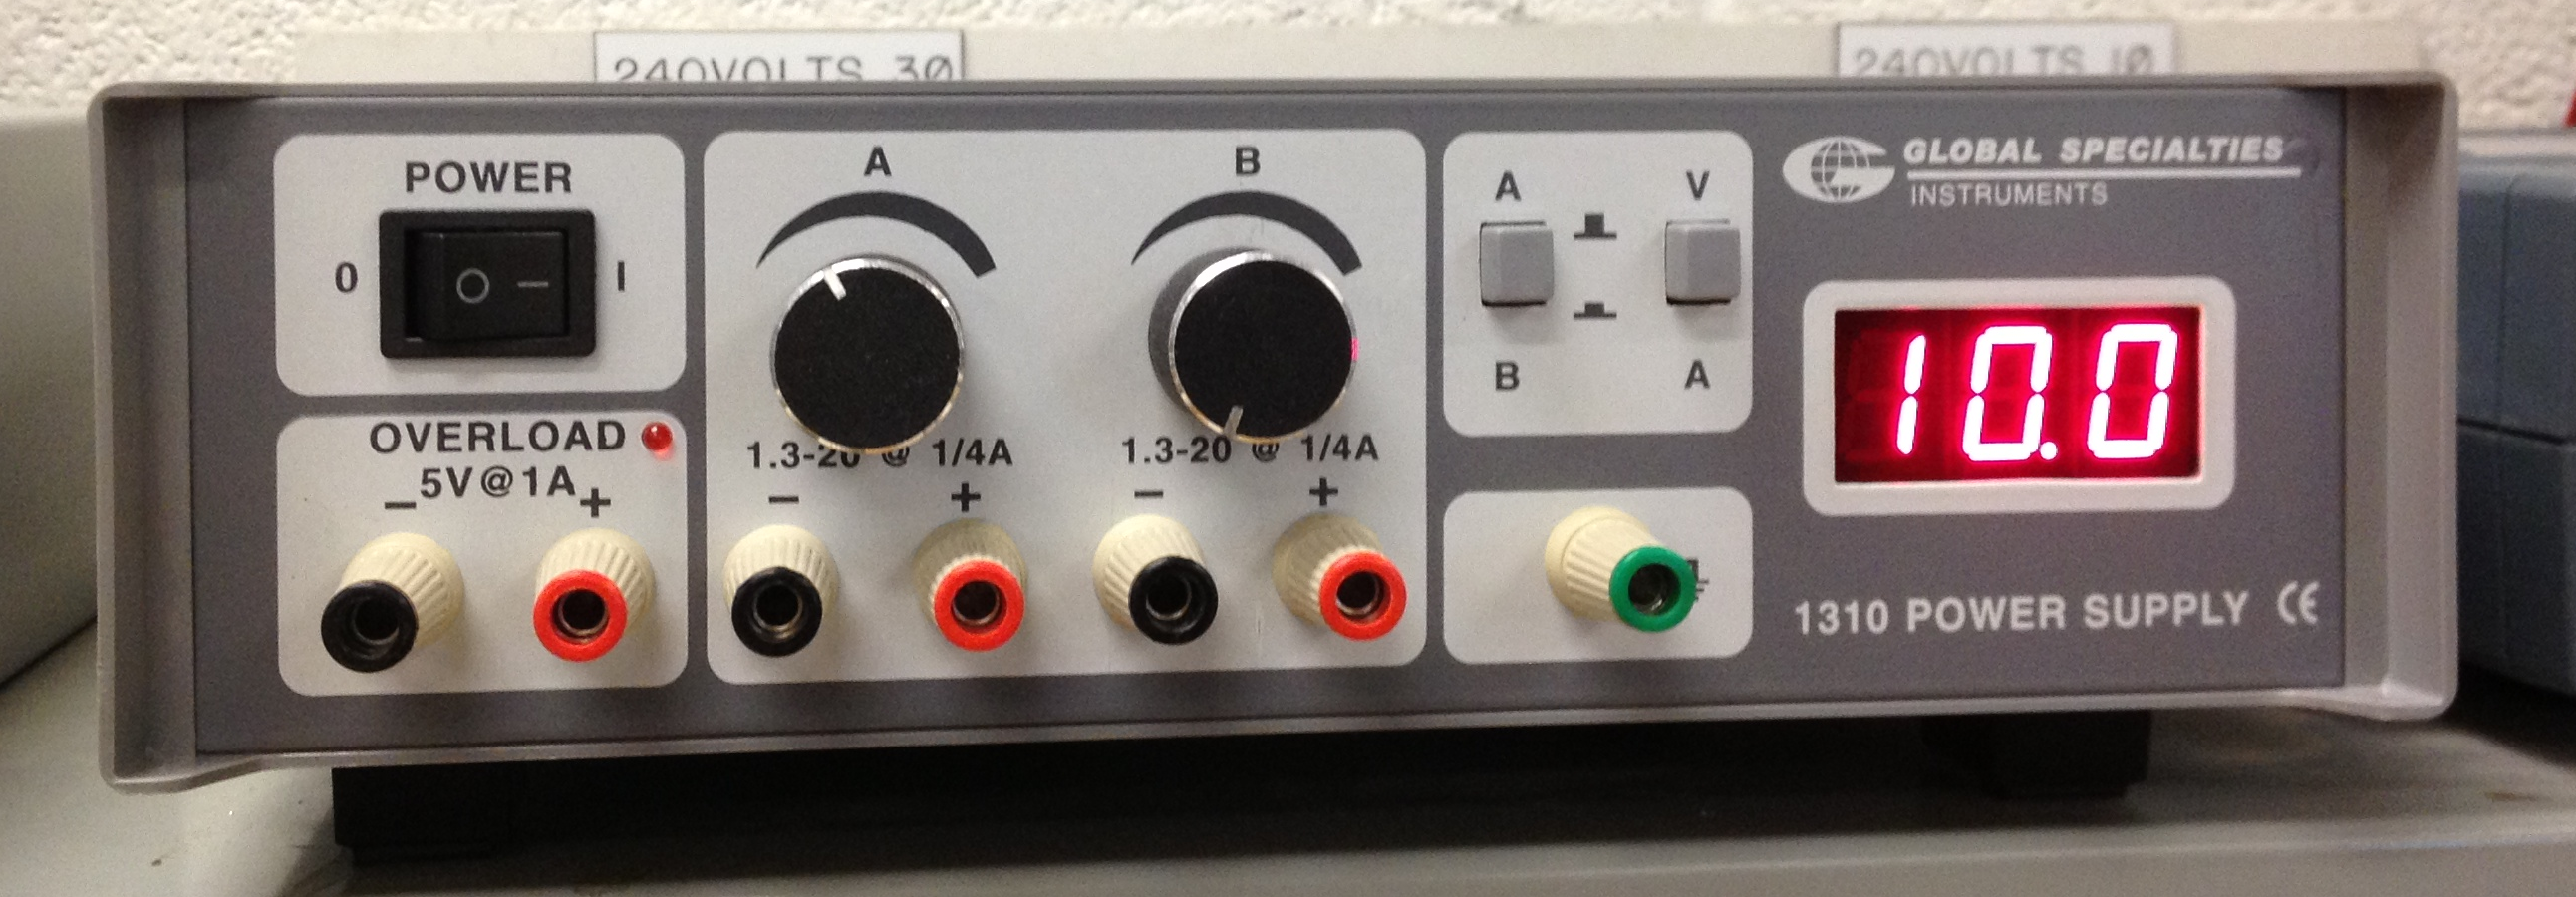
\includegraphics[width=0.7\linewidth]{Lab2_GlobalSpecialties1310}
\caption{Global Specialties 1310 Independent Power Supply}
\label{fig:Lab2_GlobalSpecialties1310}
\end{figure}

Figure \ref{fig:Lab2_TektronixCDM2050DigitalMultimeter}: The Tektronix CDM250 Bench top Digital multimeter instrument is used to measure voltage, current, resistance, capacitance, frequency, and diodes among other things. \textbf{Leave the wires attached to this meter, the connectors are unique and hard to find.}\\

\begin{figure}
\centering
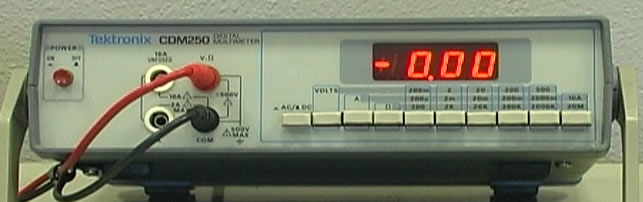
\includegraphics[width=0.7\linewidth]{Lab2_TektronixCDM2050DigitalMultimeter}
\caption{Tektronix CDM250 Digital Multi Meter (DMM).}
\label{fig:Lab2_TektronixCDM2050DigitalMultimeter}
\end{figure}


Figure \ref{fig:Lab2_Multimeters}: The Cen-tech multimeters are standard DMMs. The left meter can also measure transistor values, and test 1.5 and 9V batteries. The center meter adds temperature (with a thermocouple probe), frequency, as well as capacitance. The Fluke 87 Digital Multimeter measures Voltage, Current, Resistance, Continuity, with holding function.  True RMS stands for true Root Mean Square, which is an accurate measure of the power that an AC signal can produce.\\

\begin{figure}
\centering
\includegraphics[width=0.7\linewidth]{Lab2_Multimeters}
\caption{Left and center, Cen-tech multimeters. Right Fluke 87 Digital Multimeter, a True RMS meter.}
\label{fig:Lab2_Multimeters}
\end{figure}

Figure \ref{fig:Lab2_Instek_SFG2004_FunctionGenerator}: The Instek SFG2004 function generator is used to produce square, triangular, and sine waves at frequencies from 1 to 100 kHz.\\

\begin{figure}
\centering
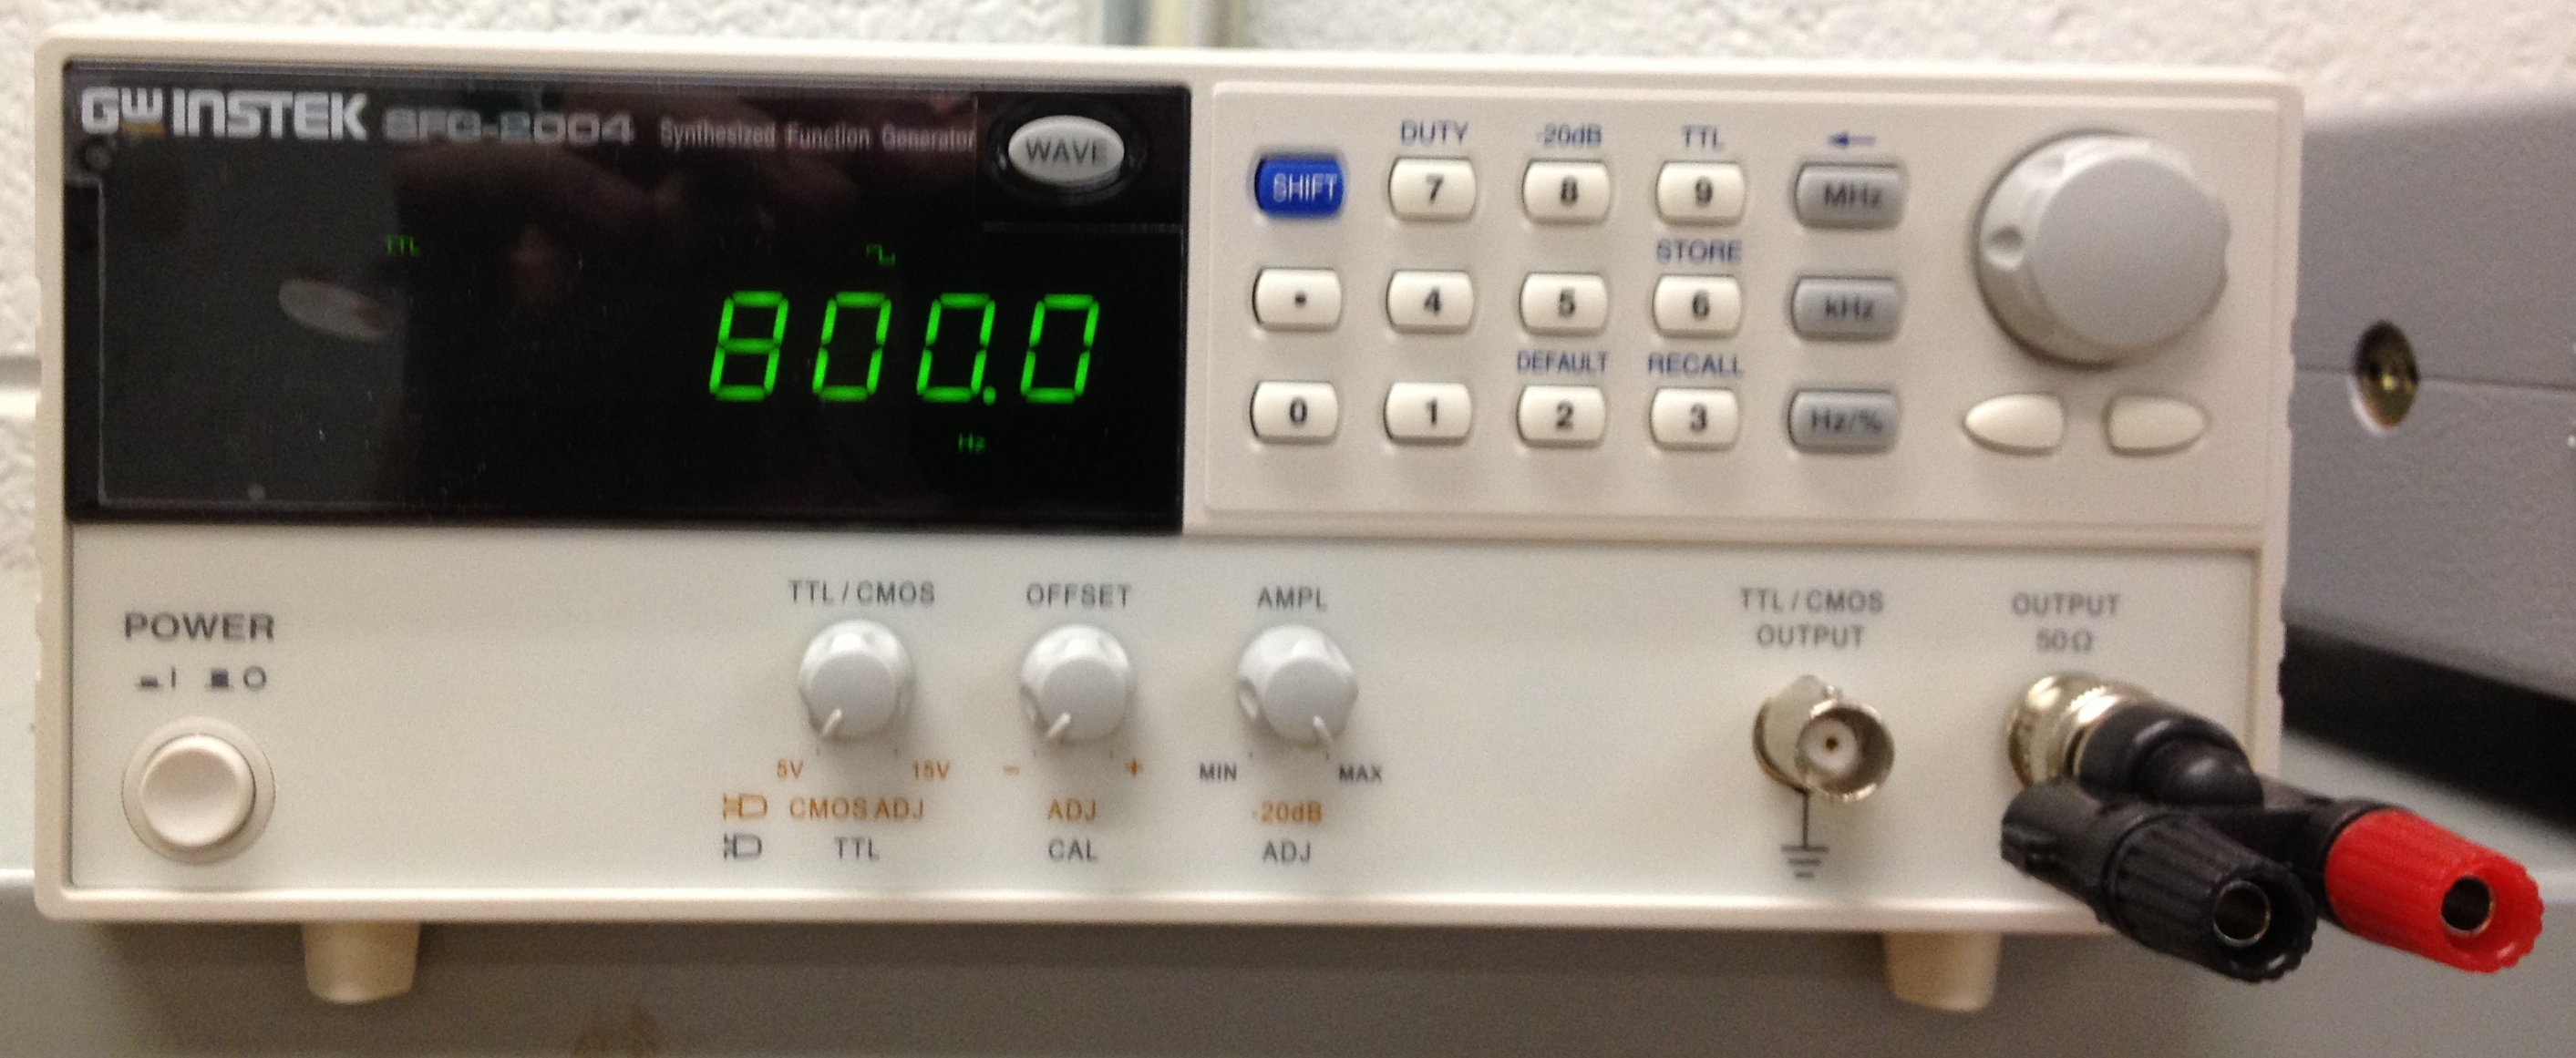
\includegraphics[width=0.7\linewidth]{Lab2_Instek_SFG2004_FunctionGenerator}
\caption{Instek SFG 2004 Function Generator.}
\label{fig:Lab2_Instek_SFG2004_FunctionGenerator}
\end{figure}


Figure \ref{fig:Lab2_Tektronix1002_Oscilloscope} The Tektronix 1002 Dual Channel 60 MHz Digital Storage Oscilloscope is used to observe and measure dynamic signals.  There are 2 probes with the scope.  The probes attenuate incoming voltages by a factor of 1 or 10 (check this). The user manual can be found \href{http://abe-research.illinois.edu/Faculty/grift/ABE425_2016/Specs/tds1002_user_manual.pdf}{here}.

\begin{figure}
\centering
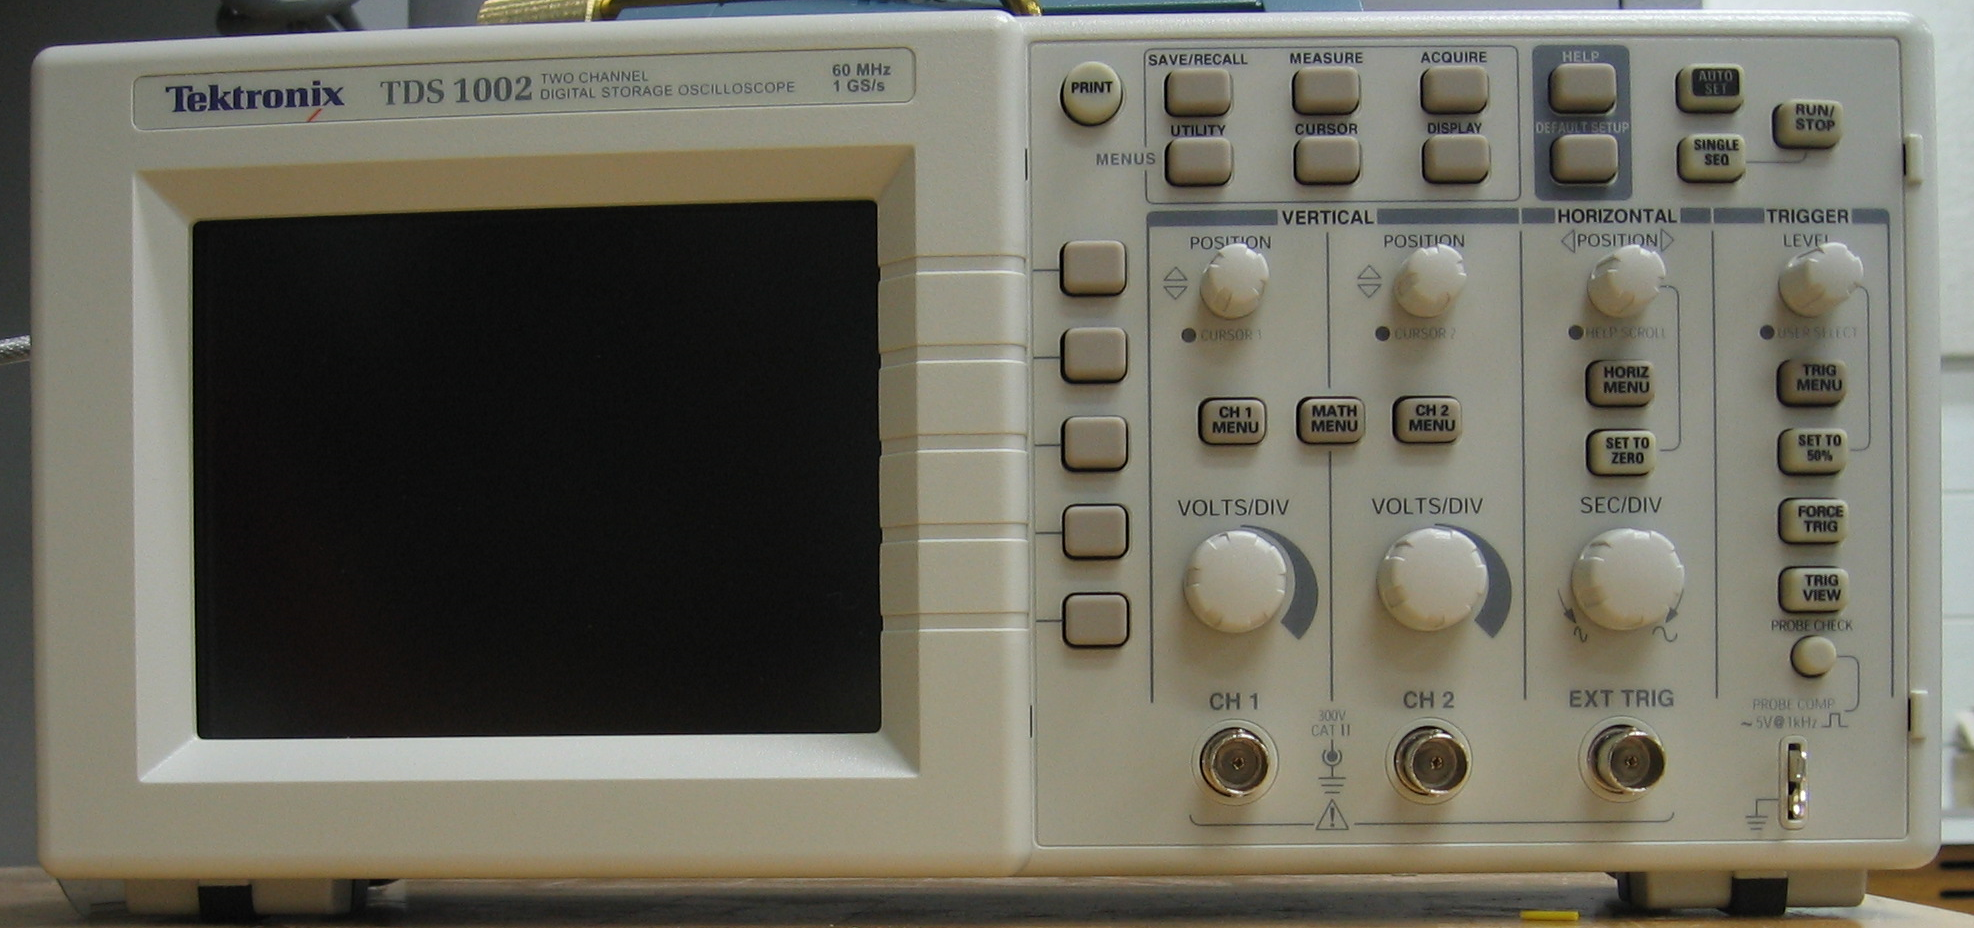
\includegraphics[width=0.7\linewidth]{Lab2_Tektronix1002_Oscilloscope}
\caption{Tektronix 1002 Dual Channel, 60 MHz Digital Storage Oscilloscope.}
\label{fig:Lab2_Tektronix1002_Oscilloscope}
\end{figure}

\begin{center}
WHEN YOU ARE DONE WITH THE LAB, MAKE SURE TO PUT THE PROBES BACK IN THE PLASTIC BAG WITH THE HOOK CAPS ATTACHED, DO NOT LEAVE ANYTHING ATTACHED TO THE SCOPE.
\end{center}

Figure \ref{fig:Lab2_NationalInstrumentsUSB6009}: The National Instruments USB 6008 Data Acquisition Module is a low-cost generic data acquisition unit, capable of Analog Input (8 inputs in Single Ended mode, 4 in Differential mode), Digital IO (12 I/O) and an event counter. The User Guide and Specs can be found \href{http://abe-research.illinois.edu/Faculty/grift/ABE425_2016/Specs/USB6008.pdf}{here}.\\

\begin{figure}
\centering
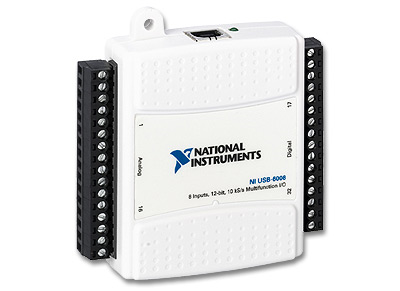
\includegraphics[width=0.7\linewidth]{Lab2_NationalInstrumentsUSB6009}
\caption{National Instruments USB 6008 Data Acquisition Module.}
\label{fig:Lab2_NationalInstrumentsUSB6009}
\end{figure}

There are some miscellaneous tools and supplies that will be used in both regular lab exercises and in the lab project.  Additional supplies will be provided as needed or can be found in the storage cabinets in the lab. When plugging in equipment it is best to use the outlets located just under the top shelf.  The ground terminals of these outlets are all connected. Power to this strip of outlets is controlled by a breaker switch under the shelf to the side of the bench.  A red light on the top shelf shows whether the power is on.

\section{Procedures}

Generate a sinusoidal pulse with a frequency of 1000 Hz and an amplitude of 5V (10V peak-peak). Show this pulse on the scope then perform the following measurements:

\begin{enumerate}
\item Measure the peak-peak value and the frequency of this pulse using the scope (push the "Measure" button).
\item Measure the DC component of this pulse using the Digital Multimeter then adjust the offset to 0.
\item Measure the cycle RMS value using the scope.
\item Measure the RMS value using the Digital Multimeter.
\item Measure the RMS value using the RMS Digital Multimeter.
\item Measure the RMS value using the Tektronix CDM250 Digital Multi Meter (on bench).
\end{enumerate}

Repeat all the steps above for a square wave and a triangular wave. Then repeat all measurement when you have a 5V offset. Then fill out the form below.
\begin{figure}
\centering
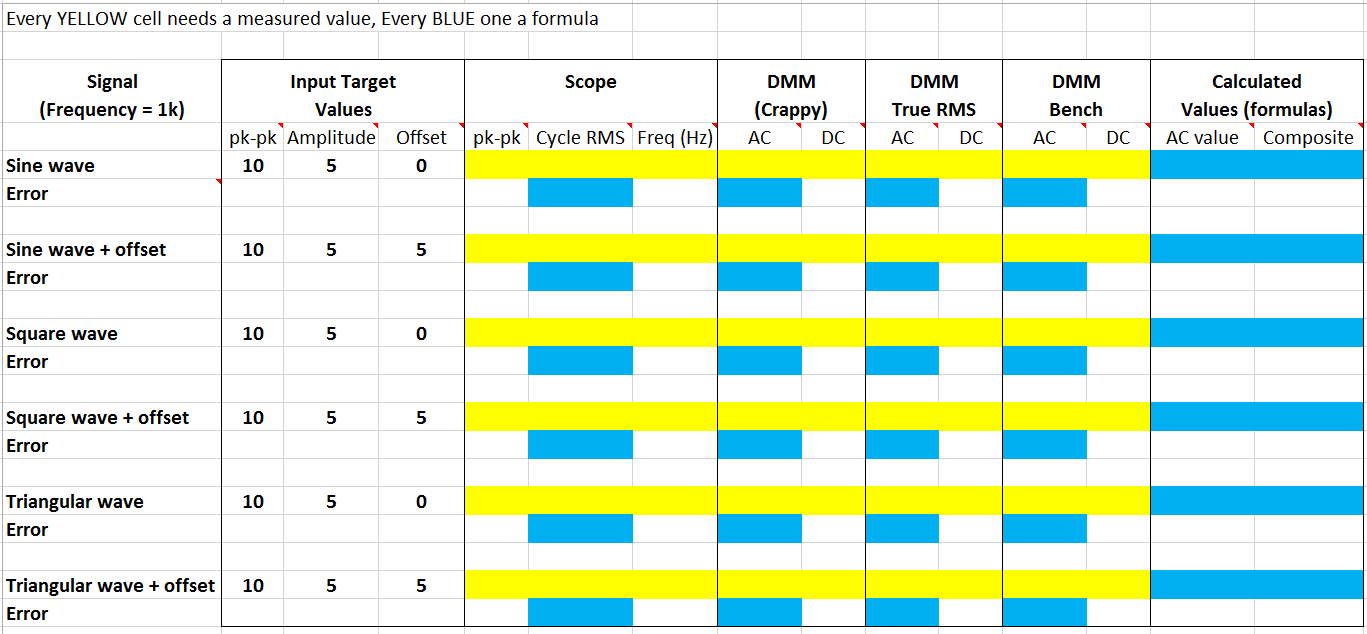
\includegraphics[width=1\linewidth]{Lab2_Table1}
\caption{ Use \href{http://abe-research.illinois.edu/Faculty/grift/ABE425_2016/Labs/Lab2_InstrumentFamiliarization/Lab2_Table1.xlsx}{this Excel spreadsheet} to record and analyze your data.}
\label{fig:Lab2_Table1}
\end{figure}

\section{Questions}

Q1: What is the purpose of a function generator?\\
A1:\\


Q2: In your results of measuring the RMS value using DMM, RMS and DMM on the bench, which one is most close to your ideal value?\\
A2:\\

\end{document}